\documentclass{beamer}

\usepackage{amsmath}
\usepackage{amsthm}
\usepackage{amsfonts}
\usepackage{amssymb,enumerate}
\usepackage{amsthm,stmaryrd}
\usepackage[all]{xy}
\usepackage{hyperref}
\usepackage{xcolor}
\usepackage{tikz}
\usepackage{scrextend}
\usepackage{apacite}
\usetikzlibrary{shapes.geometric}
\usepackage{graphicx}
\graphicspath{ {./images/} }


%
% Choose how your presentation looks.
%
% For more themes, color themes and font themes, see:
% http://deic.uab.es/~iblanes/beamer_gallery/index_by_theme.html
%
\mode<presentation>
{
  \usetheme{Madrid}      % or try Darmstadt, Madrid, Warsaw, ...
  \usecolortheme{beaver} % or try albatross, beaver, crane, ...
  \usefonttheme{default}  % or try serif, structurebold, ...
  \setbeamertemplate{navigation symbols}{}
  \setbeamertemplate{caption}[numbered]
  %\setbeamertemplate{theorems}[numbered]
  \setbeamercolor{structure}{fg=darkred}
   \setbeamercolor{block body}{bg=gray!10!white}

} 

\usepackage[english]{babel}
\usepackage[utf8x]{inputenc}
%\usepackage[utf8]{inputenc}
%\usepackage{enumitem}
\usepackage{amsmath}
\usepackage{amsfonts}
\usepackage{amssymb,enumerate}
\usepackage{amsthm,stmaryrd}
\usepackage{float}
\usepackage{graphicx}
\usepackage{verbatim}
\usepackage{subcaption}
\usepackage{mathtools}
\usepackage{fancyvrb}

\newtheorem{prop}{Proposition}
\newtheorem{protocol}{Protocol}
\newtheorem{prob}{Problem}
\newtheorem{prop1}{Proposition 1}
\newtheorem{prop2}{Proposition 2}
\newtheorem{defn}[prop]{Definition}
\newtheorem{defns}[prop]{Definitions}
\newtheorem{lem}{Lemma}
\newtheorem{ex}{Example}
\newtheorem{exs}{Examples}
\newtheorem{n}{Note}
\newtheorem{cor}{Corollary}
\newtheorem{BA}{Buchberger's Algorithm}
\newtheorem{gbc1}{GB Criterion 1}
\newtheorem{gbc2}{GB Criterion 2}
\newtheorem{gbc3}{GB Criterion 3}
\newtheorem{defsnota}{Definitions and Notation}
\newtheorem{thm}{Theorem}
\newtheorem{fainf}{Facts about Ideals in Number Fields}
\newtheorem{rmk}{Remark}
\newtheorem{aoam}{Analysis of Add and Multiply}
\newtheorem{PN}{Projective Nullstellensatz}
\newtheorem{AN}{Recall Affine Nullstellensatz}
\newtheorem{IncStep}{Inclusion Step}
\newtheorem{PC}{The Partition Class}
\newtheorem{SPIP}{Small Principal Ideal Problem}
\newtheorem{cscheme}{Somewhat Homomorphic Scheme}
\newtheorem{prf}{Proof}
\newtheorem{idea}{Idea}
\usepackage{mathrsfs}


\title[Zero Knowledge Proofs]{Zero Knowledge Proofs}
\author{Alan R. Hahn}
%\institute{Technische Universit{\"a}t Kaiserslautern}
\institute{Clemson University}
\date{April 2021}

\begin{document}

\begin{frame}
  \titlepage
\end{frame}

%%%%%%%%%%%%%%%%%%%%%%%%%%%%%%%%
\begin{frame}
\begin{small}
\begin{idea}[ZKP]
Want to convince to someone that you know something without giving away information about what you know
\end{idea}

\pause
\begin{itemize}
\item Identification Schemes and Entity Authentication
\end{itemize}


\end{small}
\end{frame}

%%%%%%%%%%%%%%%%%%%%%%%%%%%%%%%%
\begin{frame}
\begin{small}



\begin{figure}
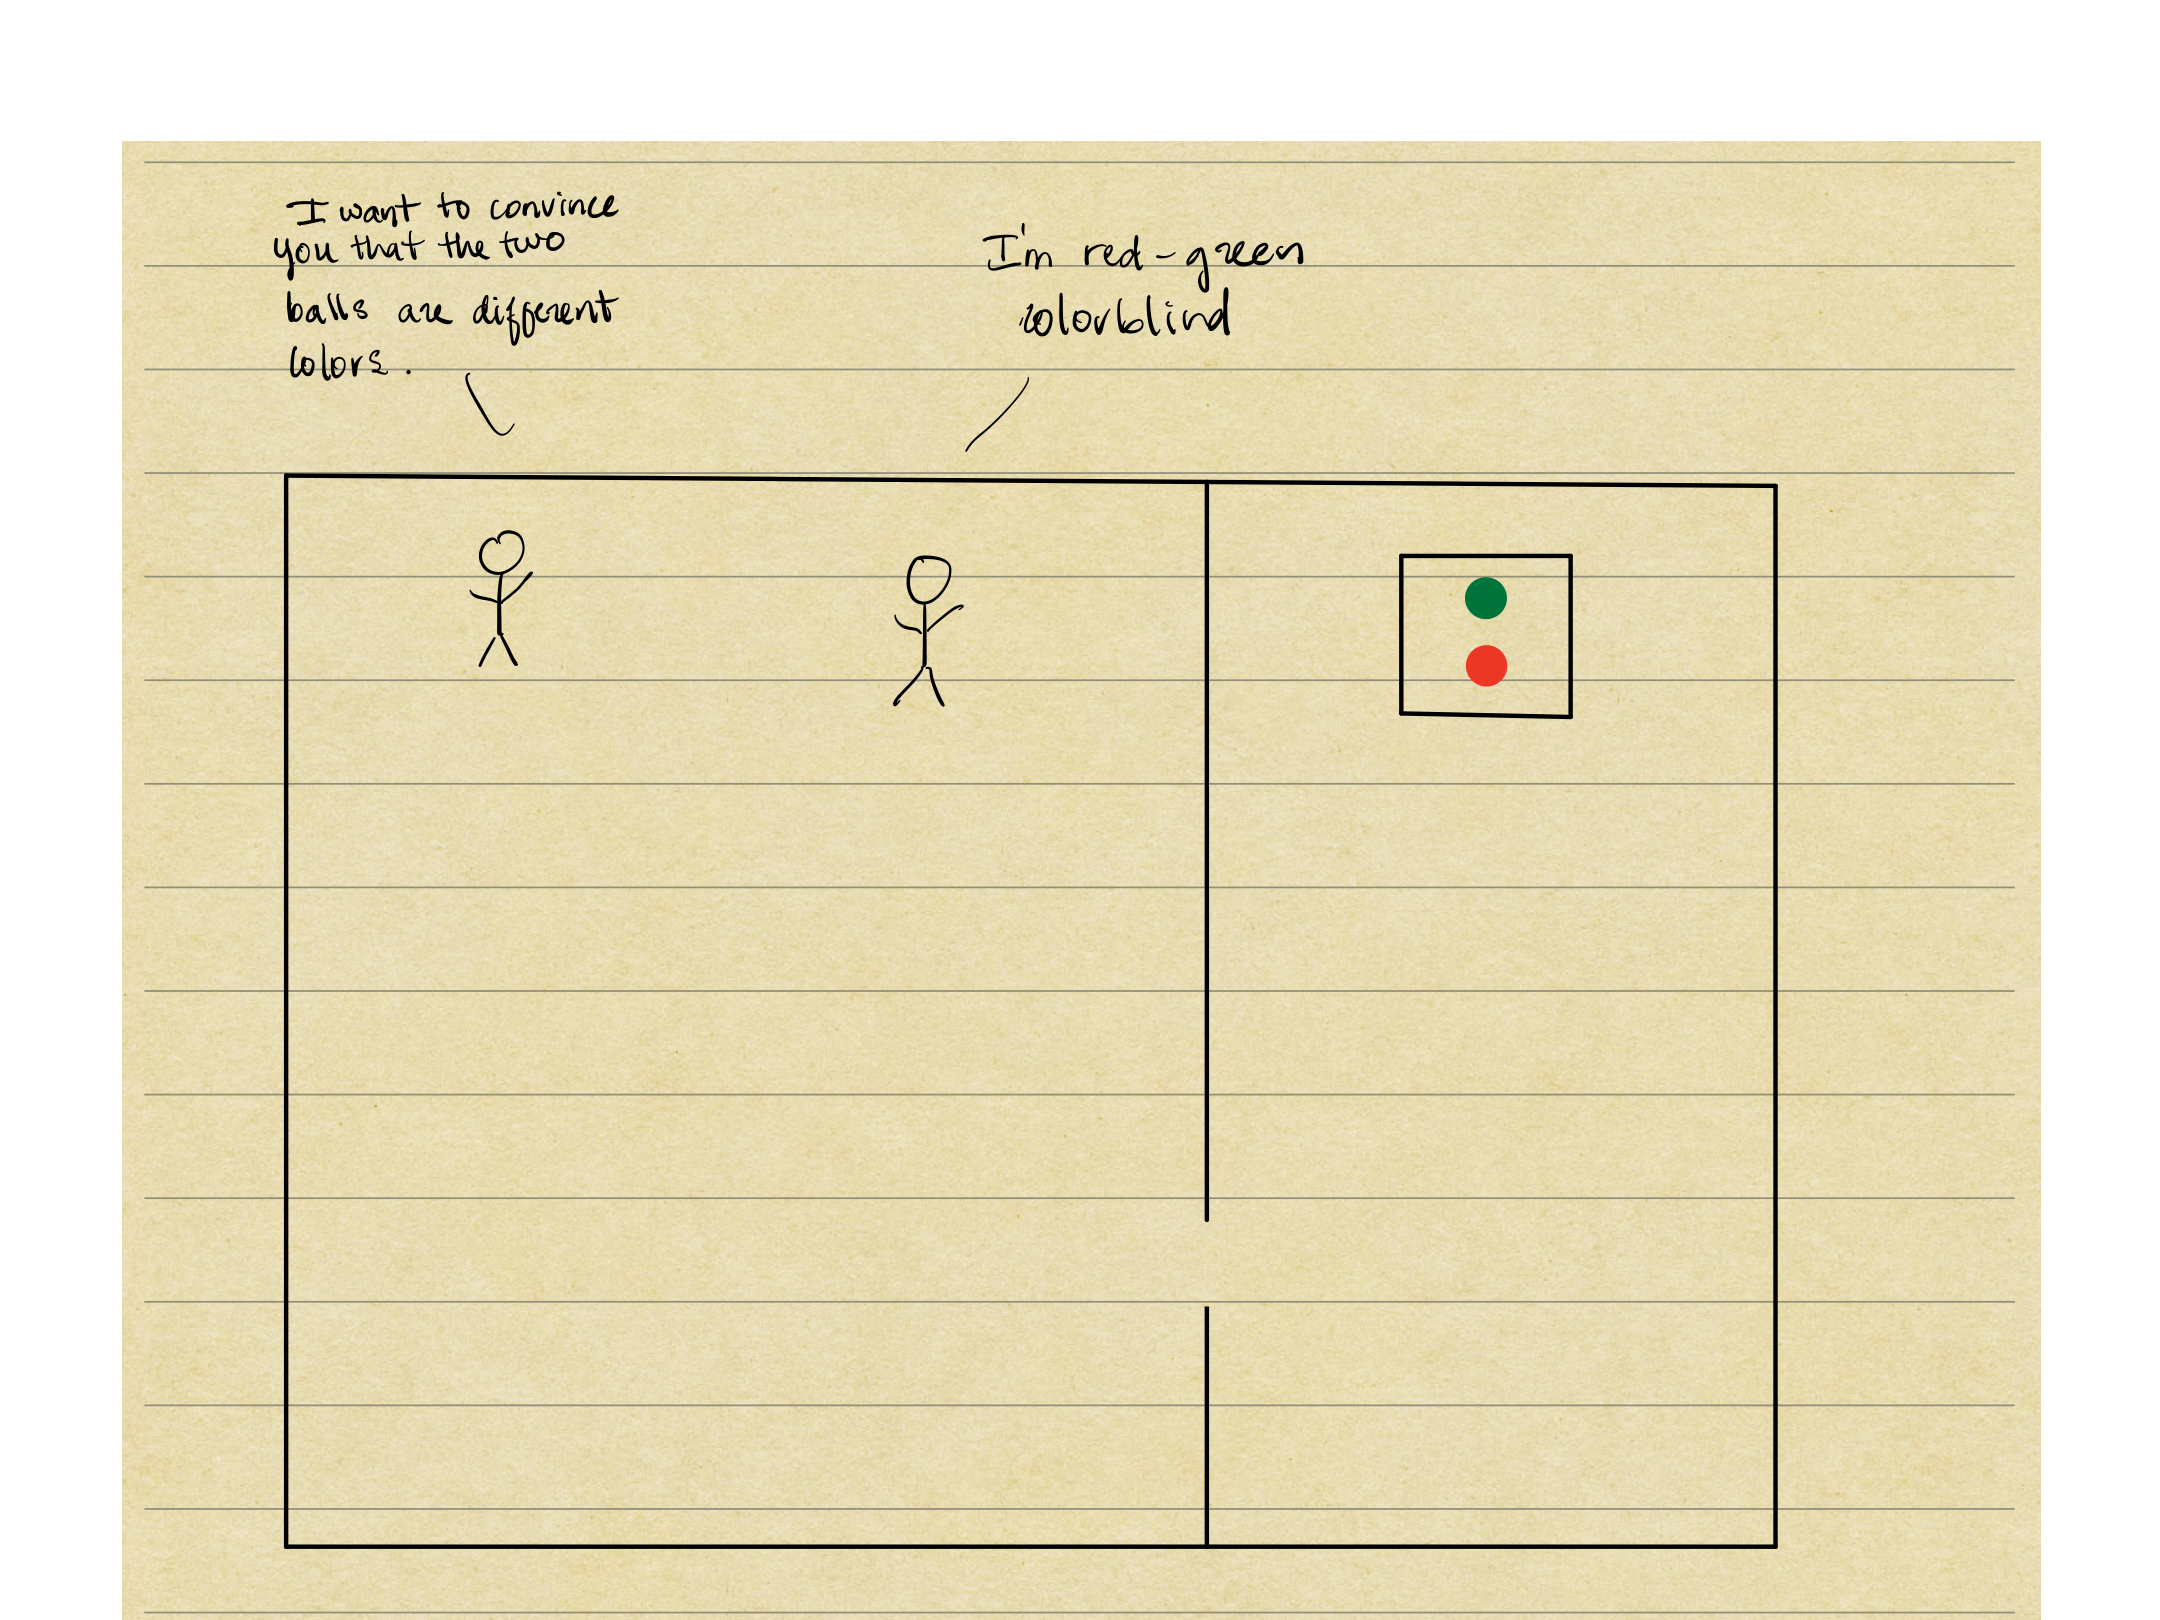
\includegraphics[scale = 0.30]{rgex}
\centering
\end{figure}


\end{small}
\end{frame}

%%%%%%%%%%%%%%%%%%%%%%%%%%%%%%%%
\begin{frame}
\begin{small}

\begin{defns}
\begin{itemize}
\item \textbf{Prover}: One proving that they have knowledge of something
\item \textbf{Verifier}: One verifying that prover really does have knowledge
\item \textbf{Completeness}: If statement is true, honest verifier will in fact be convinced it is true by honest prover
\item \textbf{Soundness}: If statement is false, no cheating prover can convince honest verifier it is true, except with small probability (soundness error)
\item \textbf{Zero Knowledge}: If statement is true, no verifier learns anything other than the fact that the statement is true
\end{itemize}
\end{defns}

\vspace{3mm}
\pause
Notes:
%\\ \hspace{5mm} - "Proof" is not the same as in the mathematical sense
%\\ \hspace{5mm} - In context of general cryptographic protocols, \textbf{Soundness} might be rephrased as \emph{"Someone who is able to impersonate the honest prover with relatively high probability must know the secret"}.
%\\ \hspace{5mm} - Can formalize above definitions/scheme through Turing machines

\begin{itemize}
\item ``Proof" is not the same as in the mathematical sense
\pause
\item In context of general cryptographic protocols, \textbf{Soundness} might be rephrased as \emph{``Someone who is able to impersonate the honest prover with relatively high probability must know the secret"}
\pause
\item Can formalize above definitions/scheme through Turing machines
\end{itemize}

\end{small}
\end{frame}

%%%%%%%%%%%%%%%%%%%%%%%%%%%%%%%%
\begin{frame}
\begin{small}
\begin{figure}
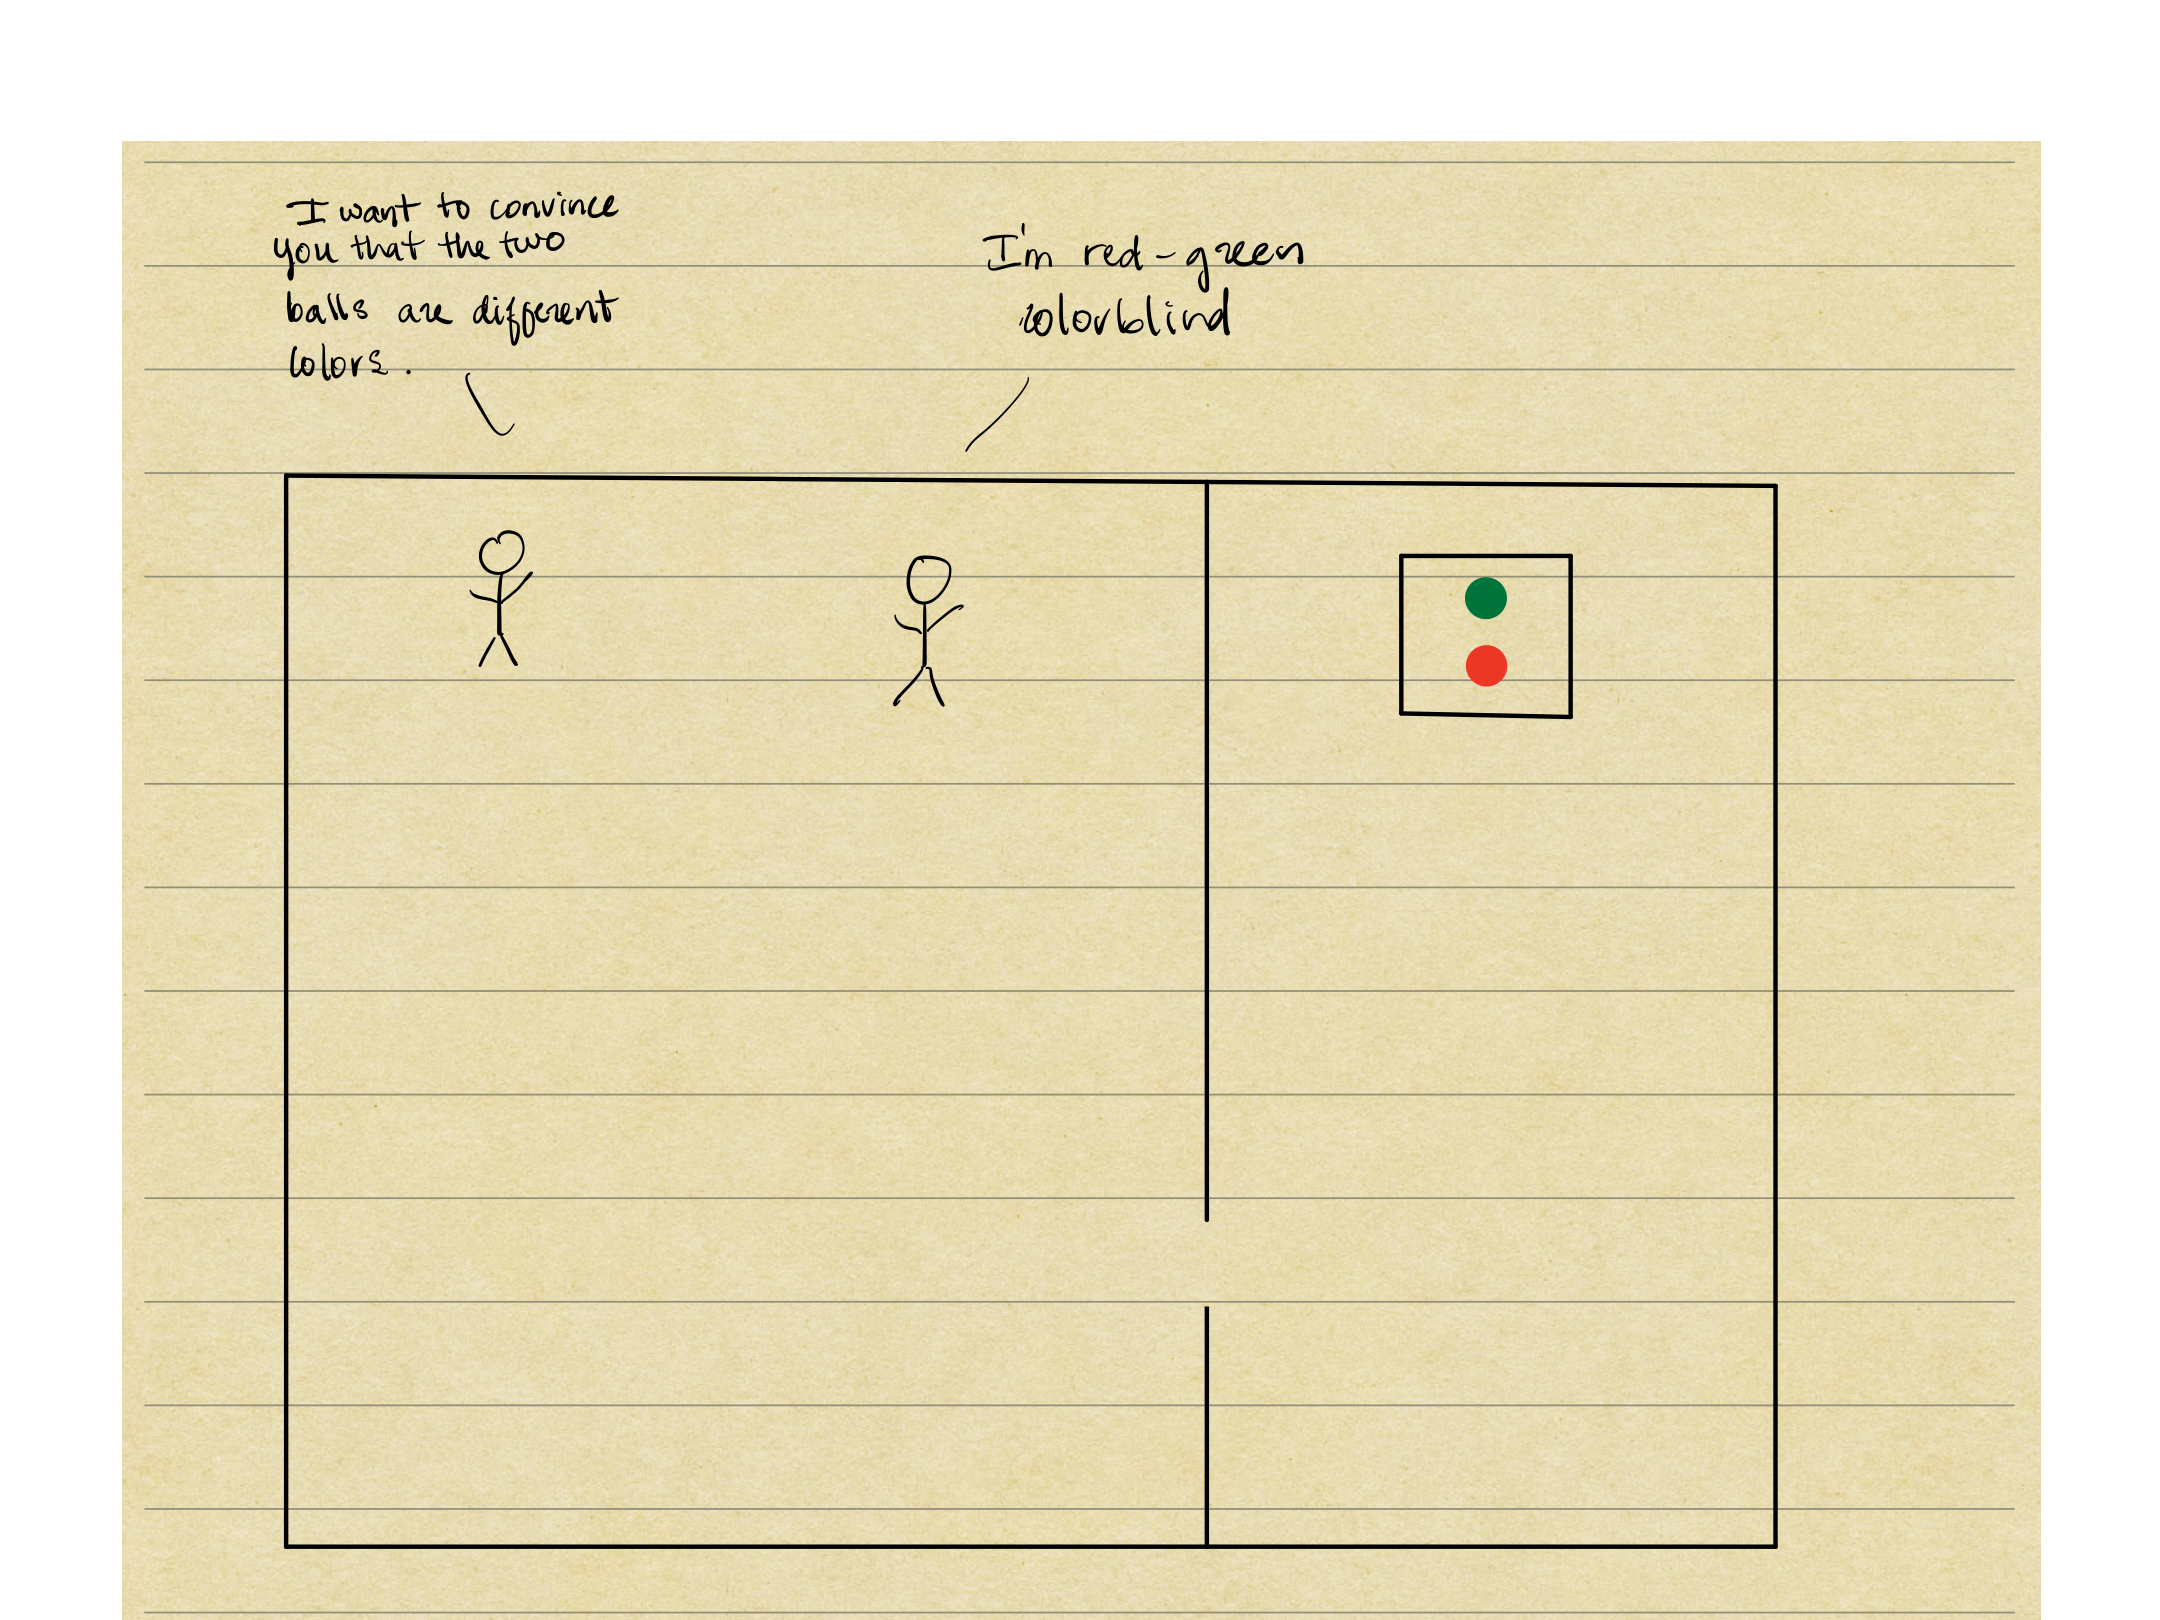
\includegraphics[scale = 0.12]{rgex}
\centering
\end{figure}
Example revisited:
\begin{itemize}
\item \textbf{Prover}: Person (you) who is trying to convince friend that the colors differ
\item \textbf{Verifier}: Friend who is colorblind
\item \textbf{Completeness}: If there really is a difference in the colors of the balls, then for a non-colorblind prover, answering ``yes" or ``no" to whether or not the ball was swapped will be trivial 
\item \textbf{Soundness}: If there was no difference in the color of the balls, then it would be hard to be correct every time (P(correct) $\sim \frac{1}{2^n}$ with $n$ trials)
\item \textbf{Zero Knowledge}: Answering ``yes" or ``no" to whether the balls were switched gives away no information to your colorblind friend about what color each ball is.
\end{itemize}


\end{small}
\end{frame}

%%%%%%%%%%%%%%%%%%%%%%%%%%%%%%%%
\begin{frame}
\begin{small}

\frametitle{Example: Feige - Fiat - Shamir Identification Scheme\\ Preliminaries}
 

\begin{prob}[Computational Composite Quadratic Residues]
Instance: A positive integer $n$ that is the product of two unknown distinct primes $p$ and $q$ where $p,q \equiv$ 3 (mod $4$), and an integer $x\in\mathbb{Z}_n^*$ such that the Jacobi symbol $\left(\frac{x}{n}\right) = 1$.
\vspace{3mm}
\\Question: Find $y\in\mathbb{Z}_n^*$ such that $y^2\equiv \pm x$ (mod $n$).
\end{prob}
\vspace{2mm}
Setup: 
\begin{itemize}
\item $n = p\cdot q$ is public while $p,q$ are private
\item Choose random $S_1, ..., S_k\in\mathbb{Z}_n$
\item For $1\leq j\leq k$, compute $I_j = \pm1/S_j^2$ (mod $n$), where the sign is chosen randomly
\item \textbf{I} $= (I_1, ..., I_k)$ is the public key and \textbf{S} $= (S_1, ..., S_k)$ is the private key
\end{itemize}



\end{small}
\end{frame}

%%%%%%%%%%%%%%%%%%%%%%%%%%%%%%%%%%
\begin{frame}
\begin{small}
\frametitle{Example: Feige - Fiat - Shamir Identification Scheme}
Recall \textbf{I} $= (I_1, ..., I_k)$ is the public key and \textbf{S} $= (S_1, ..., S_k)$ is the private key
\vspace{2mm}
\begin{protocol}[Feige - Fiat - Shamir Identification Scheme]
Repeat the following steps until verifier is convinced: 
\begin{itemize}
\item[com] Prover chooses random $R\in\mathbb{Z}_n$ and computes $X = \pm R^2$ (mod $n$) with random sign, and sends this $X$ to verifier
\item[chal] Verifier sends prover a random boolean vector \textbf{E} $= (E_1, ..., E_k)\in\{0,1\}^k$
\item[resp] Prover computes $Y = R\prod_{\{j:E_j = 1\}} S_j$ (mod $n$) and sends this to verifier
\item[verif] Verifier verifies that $X = \pm Y^2\prod_{\{j:E_j = 1\}}I_j$ (mod $n$). If so, then verifier ``accepts", otherwise verifier ``rejects".
\end{itemize}
\end{protocol}
\vspace{2mm}
\pause
The point is that the prover wants to convince the verifier that the prover does in fact know the inverses of the $S_j^2$s, meaning that the prover does know $S_j$ for each $j$, and that the prover does not want to simply tell the verifier the $S_j$s.
\end{small}
\end{frame}

%%%%%%%%%%%%%%%%%%%%%%%%%%%%%%%%%%

\begin{frame}
\begin{small}
\frametitle{Example: Feige - Fiat - Shamir Identification Scheme \\Completeness}
Recall:
\begin{itemize}
\item \textbf{I} $= (I_1, ..., I_k)$ is the public key and \textbf{S} $= (S_1, ..., S_k)$ is the private key
\item \textbf{Completeness}: If statement is true, honest verifier will in fact be convinced it is true by honest prover
\item[resp] Prover computes $Y = R\prod_{\{j:E_j = 1\}} S_j$ (mod $n$) and sends this to verifier
\item[verif] Verifier verifies that $X = \pm Y^2\prod_{\{j:E_j = 1\}}I_j$ (mod $n$). If so, then verifier ``accepts", otherwise verifier ``rejects".
\end{itemize}
\underline{\textbf{Completeness}} 
\vspace{2mm}
\\$Y^2\prod_{\{j:E_j = 1\}}I_j \equiv  (R\prod_{\{j:E_j = 1\}} S_j)^2(\prod_{\{j:E_j = 1\}}I_j)$ (mod $n$)
\vspace{2mm}
\\$\equiv R^2 (\prod_{\{j:E_j = 1\}}S_j^2I_j)) \equiv \pm R^2 \equiv \pm X$ (mod $n$)
\end{small}
\end{frame}

%%%%%%%%%%%%%%%%%%%%%%%%%%%%%%%%%%

\begin{frame}
\begin{footnotesize}
\frametitle{Example: Feige - Fiat - Shamir Identification Scheme \\Soundness}
Recall: 
\begin{itemize}
\item \textbf{Soundness}: If statement is false, no cheating prover can convince honest verifier it is true, except with small probability (soundness error)
\item[resp] Prover computes $Y = R\prod_{\{j:E_j = 1\}} S_j$ (mod $n$) and sends this to verifier
\item[verif] Verifier verifies that $X = \pm Y^2\prod_{\{j:E_j = 1\}}I_j$ (mod $n$). If so, then verifier ``accepts", otherwise verifier ``rejects".
\end{itemize}
A dishonest prover may try to guess the challenge \textbf{E} $= (E_1, ..., E_k)\in\{0,1\}^k$ ahead of time. Then given a particular \textbf{E}, choosing $X$ to fool the verifier is straight forward: 
\vspace{2mm}
\\ \underline{\textbf{Soundness}}
\\Suppose the adversary can guess ahead of time \textbf{E}, in step 1. Then the adversary chooses $X\equiv Y^2(\prod_{\{j:E_j = 1\}}I_j)$ for a random $Y\in\mathbb{Z}_n$, and sends $X$ to the verifier as the adversary's commitment. The verifier sends back the correctly guessed \textbf{E} as the challenge, and the adversary sends back $Y$ as the response. Then the verifier verifies that $Y^2(\prod_{\{j:E_j = 1\}}I_j)\equiv X$, as this was how $X$ was initially chosen by the adversary. 

\end{footnotesize}
\end{frame}

%%%%%%%%%%%%%%%%%%%%%%%%%%%%%%%%%%
\begin{frame}
\begin{small}
\frametitle{Example: Feige - Fiat - Shamir Identification Scheme \\Soundness continued}
Recall:
\begin{itemize}
\item \textbf{Soundness}: If statement is false, no cheating prover can convince honest verifier it is true, except with small probability (soundness error)
\end{itemize}
\underline{\textbf{Soundness continued}}
\\The ability of the adversary to fool the verifier depends upon correctly guessing \textbf{E} $= (E_1, ..., E_k)\in\{0,1\}^k$ ahead of time. The probability of correctly guessing $\textbf{E}$ is $\frac{1}{2^k}$, and so the probability of correctly guessing \textbf{E} for $t$ rounds of the protocol is $\frac{1}{2^{tk}}$, which is exceedingly low.

\pause
\vspace{5mm}
Final notes: 

\end{small}
\end{frame}










\end{document}